\chapter{Method and materials}


\section{Study area} % flyttet først etter AM


%https://klimaservicesenter.no/faces/desktop/article.xhtml?uri=klimaservicesenteret/klimaprofiler/klimaprofil-oslo-og-akershus
%https://klimaservicesenter.no/faces/desktop/article.xhtml?uri=klimaservicesenteret%2Fklimaprofiler%2Fklimaprofil-buskerud  
The study area (59.36-60.45° N, 9.31-11.13° E) extends over much of the southeastern parts of Norway in municipalities Flå, Krødsherad, Sigdal, Ringerike, Modum, Hole, Lier, Øvre Eiker, Asker, Oslo, Enebakk, Indre Østfold, Våler, Råde, Moss, Frogn and Vestby in Oslo and Viken counties. 
The climate has a continental character due to rain shadows of the mountain ridges from the west. 


\begin{figure}
\centering
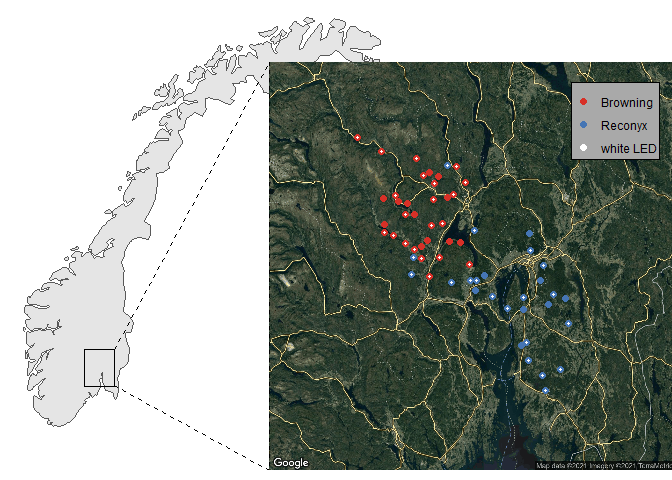
\includegraphics[width=.8\textwidth]{../R/FLM_notebook_files/figure-gfm/study-map-1.png}
	\caption[Map of study area]
	{\small
	60 sites in Southeastern Norway were included in the survey. Point colouration represents camera brand, and white dots represent sites that had periods with an additional white LED camera trap.}
\label{fig:map}
\end{figure}

The mean annual temperatures ranges from 2-6 \celsius , precipitation lies between 700-1500mm and growing season length lies between 170-190 days \autocite{Moen1999}.
Topography is predominantly flat towards the south, and more rugged and elevated towards the north. The landscape is a mosaic of forest and agricultural areas, divided with a wide network of gravel roads.
The area is situated in the southern boreal and boreonemoral zones. %Må finne oppdaterte data (frå Norges vassdrags- og energidirektorat, 2019?)
Norway spruce (\textit{Picea abies}) and Scots pine (\textit{Pinus sylvestris}) make up the dominating boreal coniferous forests, with frequent presence of silver birch (\textit{Betula pendula}) and downy birch (\textit{Betula pubescens}), then aspen (\textit{Populous tremula}), alder (\textit{Alnus incana}) and black alder (\textit{Alnus glutinosa}).



\section{Study design} 

%%%%%%%%%% Flytta av JO til metode: %%%%%%%%%%%%%%%
In northern areas, like Norway, counting animal tracks on snow has been a popular method (Linnell et al. 2007). %TODO Linnell, Odden Andren Liber Andersen Moa Kvam... 2007 distance rules for minimum counts of lynx
%TODO Linnell Brøseth Odden Nilsen 2010 sustainably harvesting a large carnivore?
Snow track counts have the benefit of visible tracks, and provide a somewhat accurate dating of the tracks to the last snowfall, when old tracks fade.
However, lately the snow season in southern Norway has been variable, which makes snow track counts unpredictable and difficult to conduct at a consistent time of year \autocite{Odden2015}.
%% Camera traps
Therefore, the Norwegian Institute of Nature Research (NINA) started with camera trap (CT) surveys in 2010,  as an additional method to monitor family groups of Eurasian lynx (\textit{Lynx lynx}) in southeastern Norway  \autocite{Odden2015}. The surveys are integrated in a coordinated Scandinavian science project on lynx, called Scandlynx. 


I was given access to CTs used in the Scandlynx project, and chose 60 sites to get a substantial amount of data.
For logistical reasons, I chose the sites closest to Oslo which weren't already equipped with white LED flashes. 
Instead, these CTs were equipped with infra-red flashes, and I will refer to them as the \emph{IR CTs}.


The IR CTs had been installed on trees 1-3 m from wildlife, human or tractor paths, 20-160 cm above ground level, 100-3000 m from closest house (median 495 m).
They were set up and handled by people from NINA, and in some places by local volunteers. 
The installation of the cameras did not follow a strict protocol, nor were their locations chosen randomly. The overall placement was systematic as decided by NINA. 
Then there was a deliberately-biased placement of the CTs put up in areas where the NINA employees or local volunteers deemed it most likely to photograph lynx, and hence, based on a combination of site accessibility and expectations of animal occurrence. % slik som \autocite{Burton2015} seier skal formidlast. 


I divided the sites randomly into three groups of 20 sites.
The first group remained unchanged as a control, and the other two groups (hereby referred to as the \emph{treatment groups}) were equipped with an additional white LED camera (hereby referred to as the \emph{white LED CTs}) in alternating 3 month-periods, as illustrated in figure\vref{fig:exp_set}.
Periods when an additional white LED CT was present (and operational), I will refer to as \emph{white LED periods}.
Periods when the white LED was absent (or inactive), I will refer to as \emph{IR periods}.
All periods from the control group, I will refer to as \emph{control periods}.
Note that control periods also are periods that only had IR CTs present, but they differ from the IR periods in that there never was a white LED present at these sites.

I up all white LED CTs above the IR CTs already in place (installation examples in figure \ref{fig:cam_ex_main}).
Using an electric drill, I mounted the CTs with metal cases that remained locked between visits.
I used short logs to adjust the angle of the white LED CTs, aligning them to match the corresponding IR CT's field of view.
Vegetation obstructing the view of any camera was removed at setup, or when noticed during a later visitation (e.g. tall grass during summer).
At one site the IR camera had been installed so far above ground level that I chose to position the white LED CT below the IR CT. %Atle fjerna kryssref til bildet
The metal cases containing the white LED CTs remained at each site until the end of the survey. Note that the second treatment group had no additional metal case before the start of their first white LED period in May 2019.

\begin{figure}
	\begin{center}
		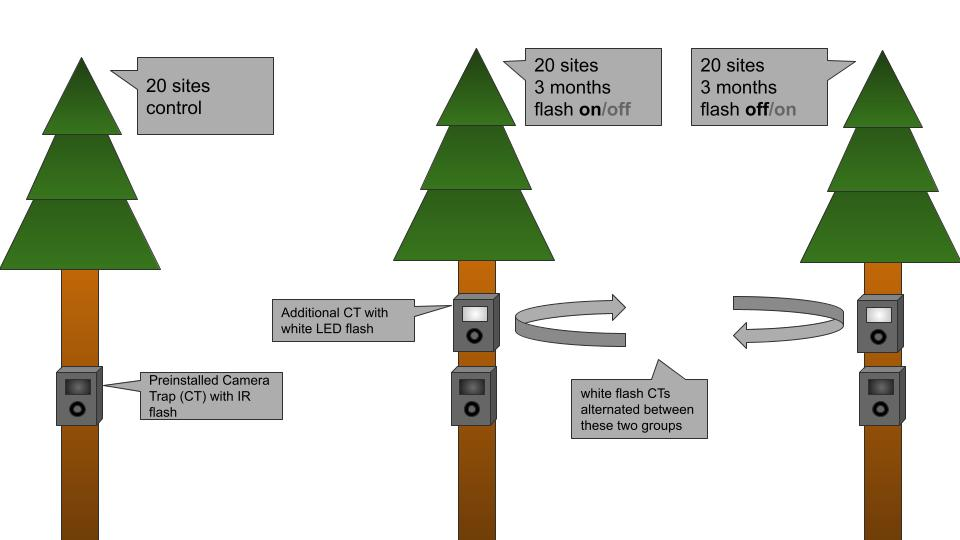
\includegraphics[width=\textwidth]{./img/cam_example/experiment_setup.jpg} %insert figure of groups     
	\end{center}
	\caption[The experimental setup]
	{The experimental setup.  \small %\par
		60 sites with preinstalled Infrared Camera Traps (IR CTs) that was divided into three groups, where the first group remained unchanged (control group), and the two other alternated on having additional white LED CTs present or not (treatment groups).}
	\label{fig:exp_set}
\end{figure} 

\begin{figure}
			\centering
			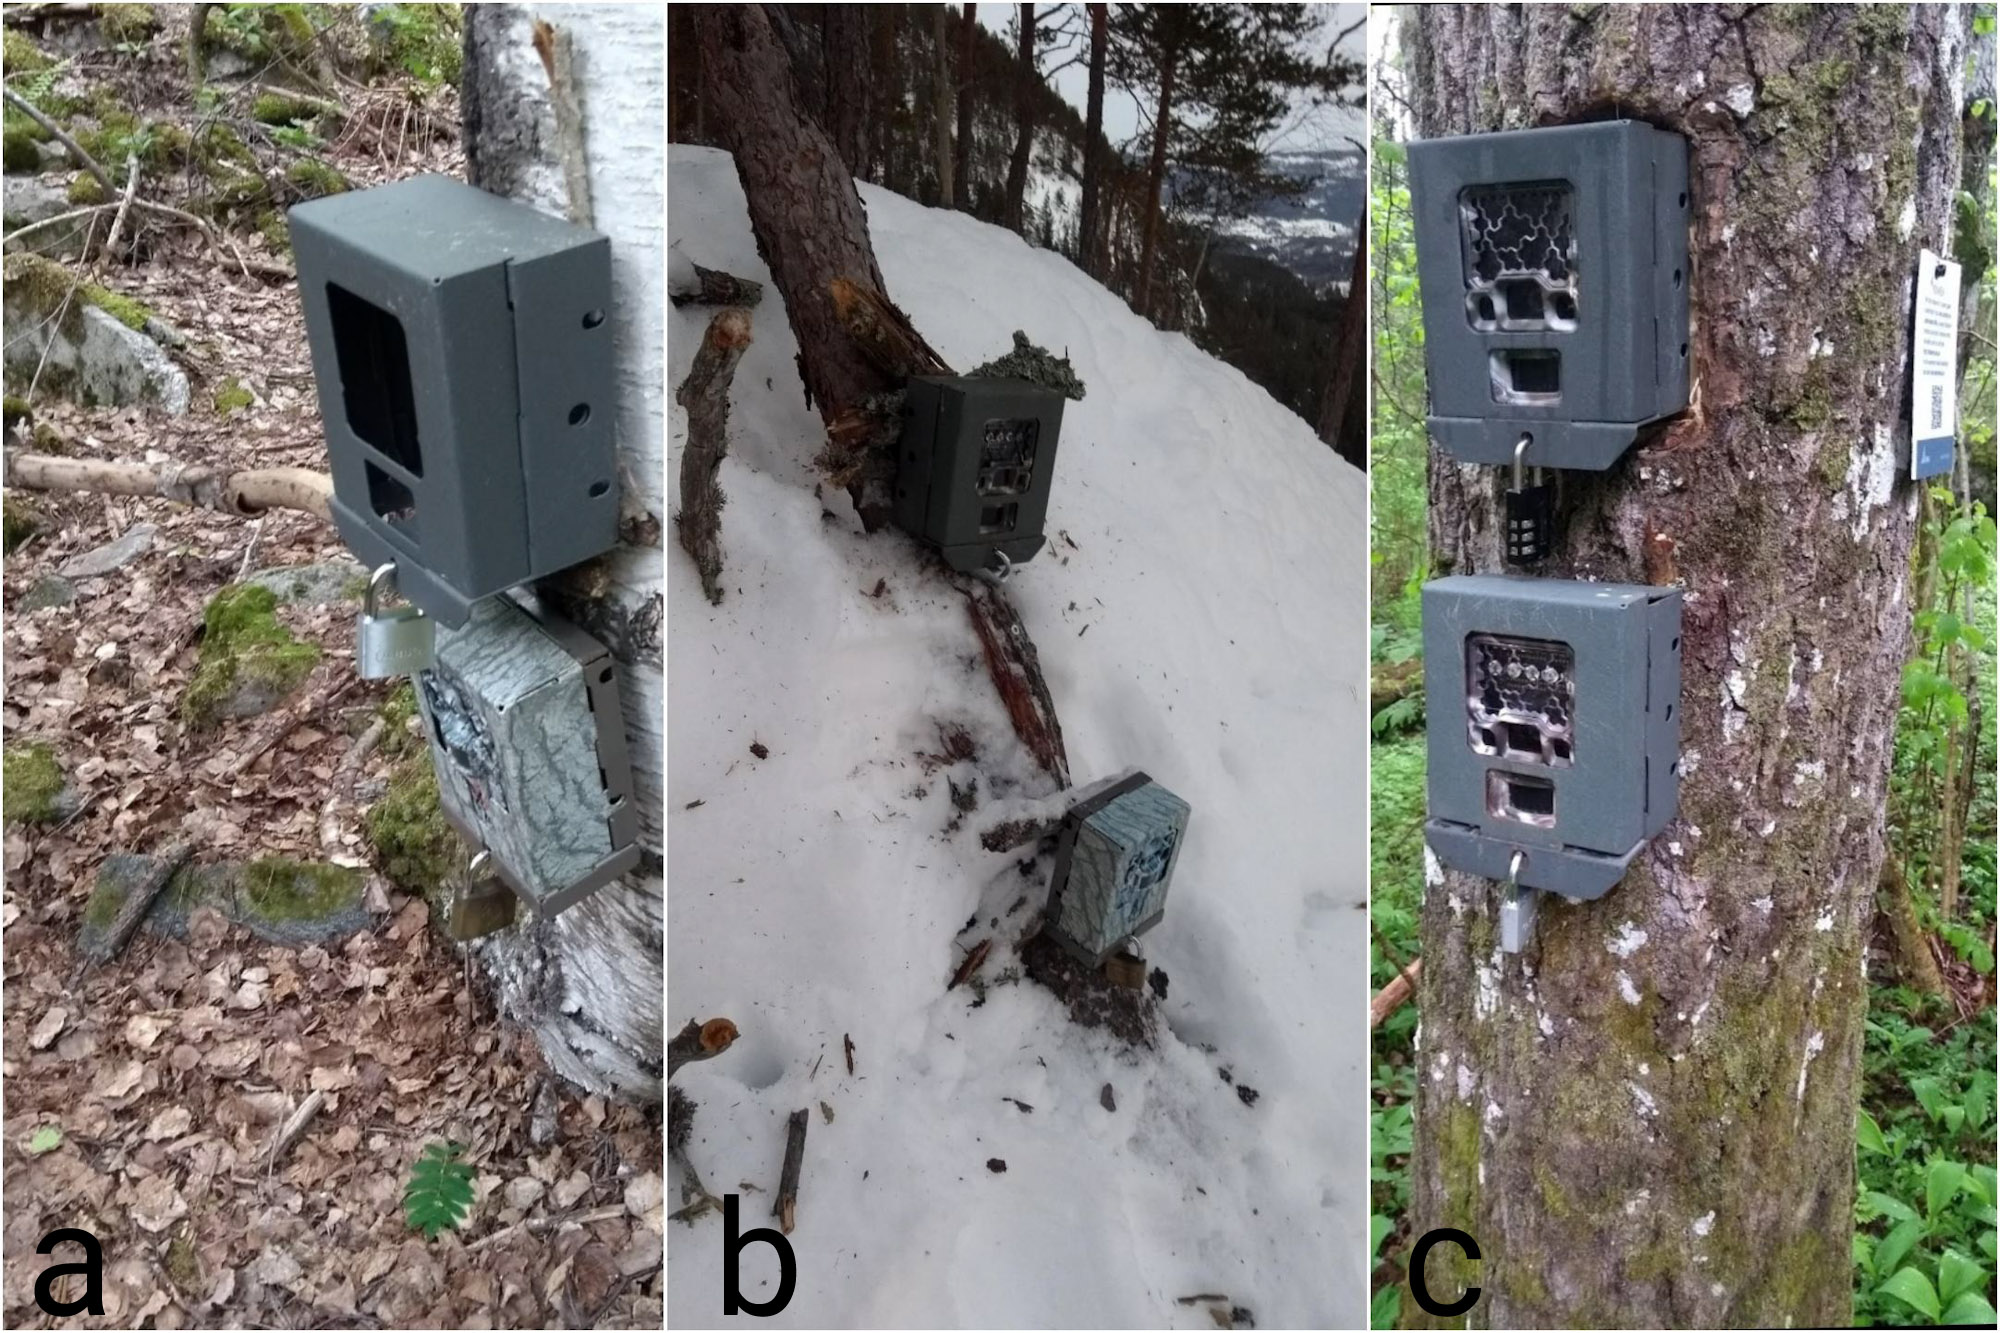
\includegraphics[width=\textwidth]{./img/cam_example/install_ex4.jpg}
			\caption[Examples of camera installations]
	{Examples of camera installations.  \small %\par
		The preinstalled IR cameras varied in the way they were set up. Lower cameras had Infra-Red flash, upper cameras had white LED flash. Additional CT boxes remained during IR periods, as seen in picture a.}
	\label{fig:cam_ex_main}
\end{figure}



I visited sites of the treatment groups at least once every three months in order to move the white LED cameras.
For logistical reasons I visited sites of the control group less often.
However, as all cameras were part of other, ongoing projects, they were occasionally visited by workers from NINA to retreive the Secure Digital memory cards (hereby SD Cards) for data. %write in full on first mention (-Atle)
This was mostly the case for sites close to, and south of, Oslo, or rather, the cameras not normally operated by local volunteers.








\section{Data Collection} 


Five different models of Reconyx (address: 3828 Creekside Ln, Ste 2, Holmen, WI 54636, USA, www.reconyx.com) cameras were used, 
and one model of Browning (address: One Browning Place, Morgan, UT 84050, USA, www.browningtrailcameras.com).
Model names and flash types are presented in table \ref{tab:cam_mod}.  
As seen in the map in figure \ref{fig:map}, there was a correlation between latitude and camera brand.
Since all Reconyx models were from the same series, they were practically identical in all aspects except for the type of flash. Differences in features and settings between the Reconyx an the Browning CTs are presented in table \ref{tab:cam_set}. For my analyses, I assumed all IR CTs to be practically identical.


Cameras were operating 24 hours per day. All were set to take photos as quickly as possible with the \emph{rapidfire} and \emph{no delay} settings. 
The two brands differed slightly in their trigger recovery speed, as shown in table \ref{tab:cam_set}.
However, the difference was not large enough to affect the results. 
More important for the result would be differences in detection area due to my placement of the white LED CTs.
Differences in horizontal angle between IR and white LED CTs could cause the white LED to trigger first, and sometimes scare the passing animal away before entering the IR CT's field of view.
Browning CTs had a slightly wider detection angle than the Reconyx CTs, which could be beneficial in minimizing the times a white LED was triggered first.
Both brands had passive infrared (PIR) motion detectors\footnote{PIR motion detectors work by detecting heat radiation (infrared light), and are triggered by moving objects that are warmer than their surroundings.} 
with ranges that far exceeded the expected travelling route. 
The largest functional difference between the two brands was in the number of photos taken per trigger. 
While Reconyx CTs were set to take 3 photos per trigger, the Browning CTs were set to 8 photos per trigger. In turn, Browning CTs tended to fill their memory cards faster in areas with sheep or cattle, and due to triggering by vegetation.
Consequently, they tended to have less active days than the Reconyx, as CTs stop taking pictures when their memory cards are full.
Adding insult to injury, the Browning CTs did not have a time lapse function, confounding the number of active days.
To approach the true number of active CT days, I assumed all Browning cameras to be functional every day, unless the camera was inactive when I visited it. In that case, I considered the camera inactive since the day of its last photo.
On the other hand, Reconyx cameras were set to take one time lapse photo per day, making it easy to verify which days they were operational.



\begin{table}[h]
\caption{Camera models included in the survey}
\label{tab:cam_mod}
\centering

\begin{tabular}{llr}
\hline
Producer  & Model name & Flash type  \\
\hline 
Browning	& Spec Ops: Extreme 					& No-glow IR \\
%\multirow{5}{2cm}{Reconyx HyperFire Series} &
			& HC500 Semi-Covert IR					& Red-glow IR \\
Reconyx		& HC600 High-Output Covert IR			& No-glow IR  \\
HyperFire 	& PC800 Professional Semi-Covert IR 	& Red-glow IR \\
Series 		& PC900 Professional Covert IR 			& No-glow IR  \\
    		& PC850 Professional White Flash LED	& White LED  \\
\hline
\end{tabular}
\end{table}


\begin{table}[h]
\caption[Camera settings and features]
{Camera settings and features %\par \small 
All Reconyx-models were part of the HyperFire series and practically identical in all aspects except for type of flash. Camera specifications are gathered from product reviews (www.trailcampro.com).}
\label{tab:cam_set}
\centering
\begin{tabular}{lcc}
\hline 
 & Browning & Reconyx \\ 
\hline 
Number of cameras 	& 34(?) 	& 26(?) \\  
Trigger speed 		& 0.43 s 	& 0.28 s \\ 
Recovery speed 		& 0.8 s 	& 0.9 s \\ 
Photos per trigger 	& 8 		& 3 \\  
Detection angle 	& 45.5$^{\circ}$ 	& 42$^{\circ}$ \\ 
Field of view 		& 40.6$^{\circ}$ 	& 42$^{\circ}$ \\  
Quiet period 		& No delay 	& No delay \\ 
Trigger interval	& Rapid fire & Rapid fire \\
Time lapse			& No	 	& Yes \\
\hline 
\end{tabular} 
\end{table}



%( CT model and settings (quiet period, SENSOR SENSITIVITY, trigger speed, photograph, burst of photographs or video, type of flash, etc.) ) %TODO add into cam_mod table







% difference between the two camera types*** 
% Assumptions: chance of detection & sp validation BROWNING > RECONYX, operational days BROWNING < RECONYX



%* Number and spacing of CTs |Hofmeester 2017 
%Mention in map figure text


%* Temperature and weather during the survey 
%Don't have that data as far as I know




\section{Data processing} 

All SD cards were delivered to NINA for data processing.
The white LED CTs were considered as external flashes, and so, \textit{only the pictures from the preinstalled IR CTs} (mounted underneath the white LED cameras) % added by JO
were sorted for species identification.
First, a facial recognition algorithm (FRA) was used to identify species on all pictures. %artificial intelligence software (AI)
Second, a human sorter reviewed the software's output, confirming all the correct identifications and rectifying the wrong ones. 
Consequently, the rate of correctly identified species has increased as the FRA sometimes detect animals that aren't easily noticed by human sorters (John Odden personal communication). 
NINA's goal is for the FRA to automatically and reliably delete pictures of humans, which has been requested from The Norwegian Data Protection Authority (Datatilsynet) (John Odden personal communication).
%Nei, vi har ikke publisert artikkel på gjenkjenningsalgoritmen. Du har jo vært med på prosessen sjøl, så jeg veit ikke om du egentlig trenger referanse her, men du kan sette inn John O som pers med og merke det, så kan han eller jeg endre det slik vi mener det bør være når vi leser gjennom oppgava di..

Third, NINA provided me with a data frame containing time stamps for every triggering of each IR CT, including all metadata from the CTs, coupled with predicted species (FRA output, with a confidence number), verified species (by human sorters), number of animals and distance from camera.
Thus, if a moose ruminated in front of a camera for 30 minutes, the data frame would include an entry for each time the moose triggered the IR CT. 
Finally, I extracted metadata from all pictures taken by the white LED CTs, and used that to define the duration of each white LED period.

Four times a site's white LED CT stopped working (eg. due to full SD card or empty batteries) before the day I came to relocate it, which can be seen as the dark blue lines transitioning to light blue outside of a field work period in figure \ref{fig:timeseries}.
Time lapse photos from the white LED CTs made dating of these stops in treatment accurate, keeping the transition to IR periods reliable. 
Whenever an IR CT stopped working during a white LED period, the rest of the period represented a data gap even if the white LED CT was functioning.\footnote{Remember that white LED CTs were considered as external flashes, and their pictures were left out of the analyses.} 
Nevertheless, inhabitant animals would still be exposed to the white flash up until the start of the following IR period.
I never experienced that both the IR and white LED CTs of a site had stopped working at the same time. 


In order to remove autocorrelation in the observations, I defined an event to be any sighting of a species that occurred more than 20 minutes after the previous sighting of the same species.
Number of individuals was not taken into account.
Ergo, I counted the number of independent times a species was observed, not the number of individuals.
My predictor variable of interest was the three different types of periods, namely IR, white LED and control periods, and how they interacted with time since deployment (ie. time since the start of each period).


When modelling the detection rates, periods of similar lengths were required.
White LED and IR periods were clearly defined, but control periods lacked a common definition for period splits, as I visited control sites less frequently than the treatment sites.
Therefore, I divided the control sites into four periods of similar lengths to that of the IR- and white LED-periods (see figure \ref{fig:timeseries}). 
%Describing in brief how coding is undertaken is useful for readers to understand the methods used in relation to the results.(Meek etal 2014)


Before the analysis, four sites were removed due to technical faults, or alike.
One site was removed from the control group, as the CT turned out to have a white LED flash, contrary to what was logged in NINA's documents.
Three sites were removed from the treatment groups, because of large or frequent gaps in the data due to technical errors, and at one site, ineffective placement of the additional white LED camera. 






\section{Statistical analysis} 

To test for effects of the white LED flash I used the R programming language \autocite{R-base}, in the RStudio IDE \autocite{RStudio}, adopting large parts of the tidyverse \autocite{tidyverse} and the easystats \autocite{easystats} frameworks along the way. 
Ensuring that all species were modelled equally (and reducing workload), I wrote code in an RMarkdown-file, using the R package knitr \cite{knitr2015}, which iteratively (re)ran all processes on subsets for each species, and stored updated plots and tables to include in the final manuscript. 
Dates were handled using the R package lubridate \autocite{R-lubridate}, and for the plots of diel patterns, I defined winter as December - February, spring as March - May, and so on. 
Plots were produced using the R packages ggplot2 \autocite{ggplot2} and sjPlot \autocite{R-sjPlot}.
The map was produced using the R package ggmap \autocite{R-ggmap}.

	\subsection*{Exploring the effect of LED flash on detection rates}
I used Generalised Linear Mixed Models (GLMM) with the glmer function from the R package lme4 \autocite{R-lme4}.
I fitted separate models for each species to avoid overly complicated models. 
Locations that had 0 observations of the modelled species were filtered out before the modelling, but for all locations that had observed the species, all periods were included.
The dependent variable was count data (number of observations per day), and I therefore assumed the error term followed a Poisson distribution ($ X \sim Pois(\lambda) $).

Although there were differences between the Browning and Reconyx IR CTs, I didn't include them as variables in my models, because they correlated with spatial and microhabitat-variables.
Instead, I included location ID and week of the year as random effects to account for differences between camera sites and seasonal changes during the year of study. 
95\% Confidence Intervals (CIs) and p-values were computed using the Wald approximation.
%I used standardized parameters (mean = 0, SD = 1) to enable comparison of effect sizes. % I don't think I did so

The main term of interest was time since deployment (continuous) interacting with type of flash period (categorical; formula: n.obs $\sim$ time.deploy $\ast$ flash).
For the sites that were equipped with an additional white LED camera, time since deployment starts from the day I visited the camera, and set up or took down the white LED.
For the sites that started with an IR period, time since deployment started at the first day of field work, or when I visited them. 
The control group’s “day 0” of time since deployment were set at points reflecting the onset of field work each time, in order to obtain periods of similar lengths to that of the white LED-locations.

I trimmed the period lengths down to a reduced maximum length, based on the median length of the IR and white LED periods, to enhance meaningful comparison (Figure 2.5).
Finally, due to large eigenvalues in the fixed effects, the model failed to converge, and an error message prompted me to rescale variables.
Therefore I divided the time since deployment-variable by ten, which solved the convergence issue.
Consequently, the time parameter estimates represent the change in detection rates per 10 days. %IMR: foreslår at du endrer annoteringen på aksene dine til å vise faktiske dager, ikke dager/10

%The model failed to converge for red squirrel. Therefore, I changed the optimizer to penalized iteratively reweighted least squares step, by setting argument nAGQ = 0 in the glmer-function. %works after filtering away detectionless locations

%AM: til analyse
The control periods should stay horizontal, representing a baseline detection rate, given that the random effects succeeded in removing seasonal variation. 
If there were any effect of the white LED, and detection rates were altered, I expect the IR period to show a regression to the norm, ie. counteracting the trend during the white LED periods.
Thus, if the white LED had a negative slope along the time axis, the IR should have a positive slope. %Further, the detection rate at the start of each period, should correspond somewhat to the detection rate at the end of the previous period. Still, that pattern could be skewed to some extent due to my visitation of each location at the start of all IR and white LED periods.
To prove an effect, white LED and IR periods have to be significantly different from each other, rather than just significantly different from the control group.
Using the R package performance \autocite{R-performance} I checked the model for overdispersion, zero-inflation and singularity, which held up in every model.




\subsection*{Equivalence test and Second Generation P-Values}
% Multiple testing i arkiv/method-ark
I used the standard significance level of $\alpha = .05$, and performed an equivalence test on my model outputs, using the function equivalence\_test from the R package parameters \autocite{R-parameters}.
In an equivalence test, model parameters are tested against a Region of Practical Equivalence (ROPE) as opposed to merely one single mean value which is done in a standard Null Hypothesis Significance Test (NHST).
Thus, rather than saying that a parameter's effect was significantly different (or not) from 0, the \emph{effect size} is also considered.
If the parameter estimate and confidence interval (CI) lies outside the ROPE, the effect is significantly and practically different from 0, and the null hypothesis is rejected.
However, if the CI is inside the ROPE, H0 is accepted, no matter if a NHST would have deemed it significantly different, because the difference is so small that there is practically no effect.
The percentage of the CI inside the ROPE is identical to the Second Generation P-Value (SGPV), which was proposed %TODO by who?
 as a way to account for all the empirical data supporting null hypotheses. %TODO Språkvask.


Inside the function equivalence\_test I used the Two One-Sided Tests (TOST) rule, where the CI is set to $1 - 2\times \alpha$. In my case that gave a CI of 0.90.\footnote{Therefore, a significant difference in a TOST differs slightly from a significant difference in a standard NHST, which is based on a CI of 0.95.}
For models from count data, the residual variance is often used to define the ROPE range. However, the description of the rope\_range function from the package bayestestR (R-bayestestR) states this threshold as "rather experimental" and that the range is probably often similar to the default [-0.1, 0.1] of a standardized parameter.
Hence, I used the default ROPE range which corresponds to a negligible effect size according to Cohen, 1988.

%In the TOST procedure, the null hypothesis is the presence of a true effect of DL or DU, and the alternative hypothesis is an effect that falls within the equivalence bounds or the absence of an effect that is worthwhile to examine. \autocite{Lakens2017}


%%%% Figurene bør havne på same side for å minimere antall fargesider

\begin{figure}[b]
	\centering
	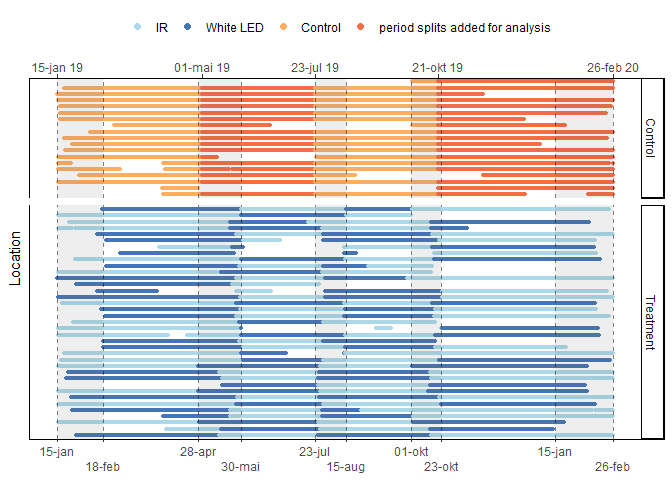
\includegraphics[width=.8\textwidth]{../R/FLM_notebook_files/figure-gfm/effort-facet-1.png}	
	\caption[An overview of active camera days]
	{\small Overview of active camera days for each camera throughout the whole study period.  
		Colours indicate the different periods for each site. White spaces indicate gaps where the IR CTs were inactive. Control camera periods were defined in similar lengths to that of the treatment group during analysis. As a result, the first day of control periods are often set at dates far from when I actually visited a site. Shaded areas represent my field work periods.}
	\label{fig:timeseries}
\end{figure}

\begin{figure}[b]
	\centering
	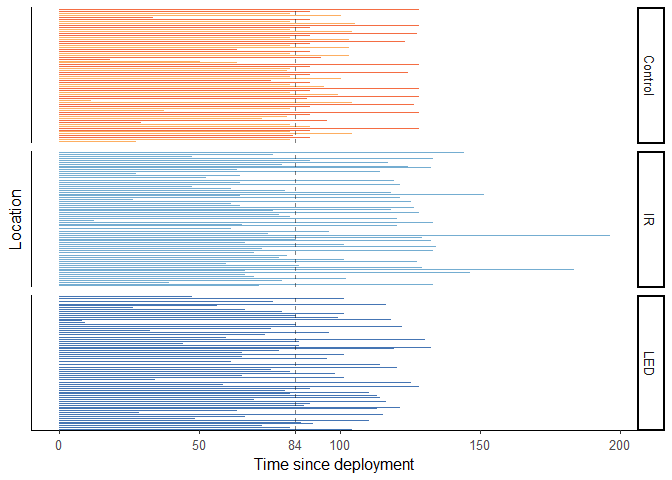
\includegraphics[width=.8\textwidth]{../R/glmm_sp_files/figure-html/period-length-wControl-1.png}
	\caption[Period lengths]
	{\small Period lengths for each camera.
		Vertical line represents the median IR period length, which was shorter than the median of the other groups. Data superseding the median were trimmed away for the GLMM.} 
	\label{fig:median_period}
\end{figure}

%%%%%%%%%%%%%%%%%%%%%%%%%%%%%%%%%%%%%%%%%%%%%%%%%%%%%%%%%%%%%







